\subsection{Predicting Core Composition}

\vspace{2mm}
\begin{figure}
  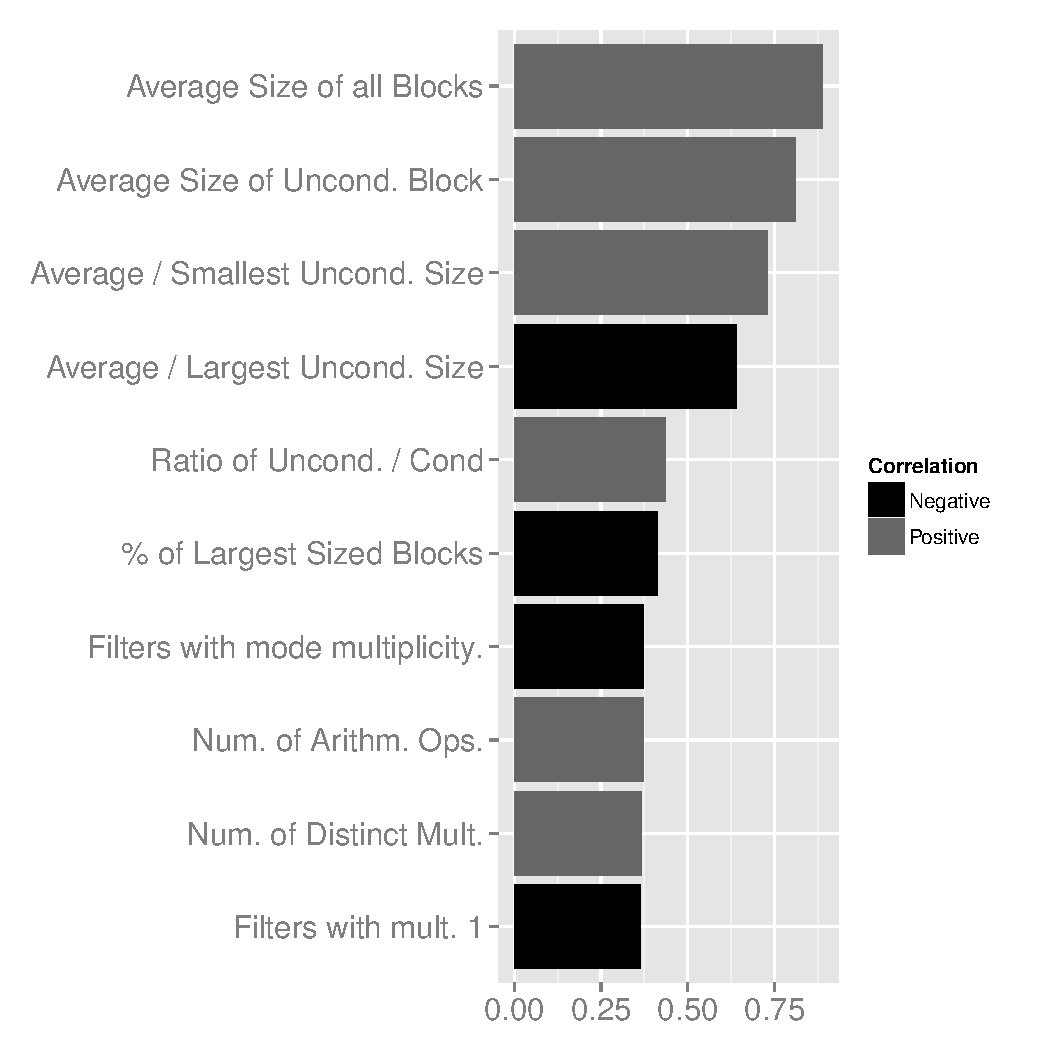
\includegraphics[width=0.51\textwidth]{streamit-paper/graphics/coreCorr.pdf}
  \caption{The ten highest correlating features with the optimal number of cores.}\label{fig:corrCore}
  \vspace{4mm}
\end{figure}
\paragraph{Gathering Training Data}
Given that the optimal number of cores for a thread is independent of the number of threads found in the program, we only use the single threaded versions to determine the optimal number of cores.
For example, all benchmarks will only have a single core per thread when the application is partitioned in 15 threads as this is the maximum amount of cores that may be given to each thread rather than it being the optimal solution. 
We include multiple versions of the benchmarks using different amounts of unrolling.
To determine the optimal number of cores we only select training data that has a performance within 1\% of the best. 
  \vspace{2mm}

\paragraph{Analyzing Features}

Figure~\ref{fig:corrCore} shows the highest correlating features with the optimal number of cores.
The features are very different from the ones presented in Figure~\ref{fig:corr} and overall there are higher correlating features.
The highest correlating value has a correlation factor of 0.88 which represents the number of operations found in a basic block of code.
The second feature is similar but only takes into account blocks that will be executed unconditionally, we have chosen to exclude blocks found in loops for this metric as there is still some form of condition for those blocks to be executed.
The next two feature compare the size of the average size of an unconditional block to the largest and smallest unconditional block.
The fifth feature measures the ratio of the number of unconditional blocks to conditional.

Overall there are no features distinct to StreamIt, such as pipelines or splitjoins that correlate highly with the optimal number of cores.
We can thus infer that the optimal number of cores is independent of the structure of a StreamIt program.
Instead, it is more dependent on the amount of computation.

EDGE architecture's ability to fetch atomic instruction blocks and out-of-order execution encourages the focus on determining how much speculation is extracted from each filter.
Unfortunately StreamIt programs do not tend to have a large quantity of conditional statements and when they do they tend to be quite small.
This statement is reinforced by the correlation between the average number of conditional blocks with the optimal number of cores, which is only 0.2, compared to 0.809 for the average size of unconditional blocks.
We thus do not focus on using any speculative features from the StreamIt graph.
\vspace{2mm}

\paragraph{Linear Regression Model}
Given that the optimal number of cores is highly correlated with a few features, a linear regressor is a natural choice to predict the best number of threads.
Figures~\ref{fig:maxav} represent how the first three highest correlating values affect the number of cores.
This figure was obtained by finding the best number of cores for a single threaded benchmark.
It is important to note that the top right corner points will always be flat as we can only allocate a maximum of 15 cores.

\vspace{-2mm}
